\documentclass[11pt, a4paper]{article}
\usepackage[margin=2.4cm]{geometry}
\usepackage[T1]{fontenc}
\usepackage{lmodern}          % fontes vetoriais Type 1
\usepackage{cmap}             % ToUnicode CMap -> texto e acentos copiaveis
\usepackage[utf8]{inputenc}
\usepackage[brazil]{babel}
\usepackage{amsmath, amssymb, amsthm}
\usepackage{bm}
\usepackage{mathtools}
\usepackage{enumitem}
\usepackage{booktabs}
\usepackage{array}
\usepackage{xcolor}
\usepackage{titlesec}
\usepackage{parskip}
\usepackage{hyperref}
\usepackage{fancyhdr}
\usepackage{tcolorbox}
\usepackage{graphicx}
\tcbuselibrary{skins, breakable}

\definecolor{darkblue}{RGB}{15,55,115}
\definecolor{midblue}{RGB}{30,100,180}
\definecolor{theorybg}{RGB}{245,250,255}
\definecolor{questionbg}{RGB}{255,252,240}
\definecolor{evencolor}{RGB}{60,0,100}
\definecolor{rubricbg}{RGB}{248,246,252}

\hypersetup{colorlinks=true, linkcolor=darkblue, urlcolor=midblue,
  pdftitle={Resolucao --- Lista de Exercicios 2 --- Macroeconomia I MPE Insper},
  pdfauthor={Macroeconomia I --- MPE Insper 2026/T3}}

\setlength{\headheight}{14pt}
\pagestyle{fancy}
\fancyhf{}
\renewcommand{\headrulewidth}{0.4pt}
\fancyhead[L]{\small\textcolor{darkblue}{\textit{Macroeconomia I --- MPE Insper --- 2026/T3}}}
\fancyhead[R]{\small\textcolor{darkblue}{\thepage}}
\fancyfoot[C]{\small\textcolor{gray}{Resolução --- Lista de Exercícios 2}}

\titleformat{\section}[block]
  {\large\bfseries\color{darkblue}}{}{0pt}{}
  [\vspace{2pt}\color{darkblue}\rule{\textwidth}{1.5pt}\vspace{4pt}]

\tcbset{
  theorybox/.style={
    enhanced, breakable, colback=theorybg, colframe=darkblue,
    fonttitle=\bfseries\small, coltitle=white, boxrule=0.5pt, arc=3pt,
    left=6pt, right=6pt, top=4pt, bottom=4pt,
  },
  questionbox/.style={
    enhanced, breakable, colback=questionbg, colframe=gray!60,
    fonttitle=\bfseries\small, coltitle=black, boxrule=0.4pt, arc=2pt,
    left=6pt, right=6pt, top=4pt, bottom=4pt, title={\textit{Enunciado (original, em inglês)}},
  },
  rubricbox/.style={
    enhanced, breakable, colback=rubricbg, colframe=evencolor!70,
    fonttitle=\bfseries\small, coltitle=white, boxrule=0.4pt, arc=2pt,
    left=6pt, right=6pt, top=4pt, bottom=4pt, title={Onde estão os pontos},
  },
}

\newcommand{\passo}[1]{\medskip\noindent\textbf{#1}\par\nobreak}
\newcommand{\intuicao}[1]{%
  \medskip\noindent\textcolor{midblue}{\textbf{Intuição econômica.}} #1\par}
\newcommand{\refbib}[1]{%
  \medskip\noindent{\small\textcolor{gray!60!black}{\textbf{Ref:} #1}}\par}
% Destaque de resposta. Precisa funcionar em texto E em modo matematico: \textbf
% sozinho quebra dentro de $$...$$ (com \frac, \approx), e \bm estoura a memoria
% do TeX quando o argumento contem \text{...}. Em matematica, so a cor -- que ja
% basta como destaque e nao depende de existir versao negrito do simbolo.
\newcommand{\resp}[1]{%
  \ifmmode {\color{darkblue}#1}\else\textcolor{darkblue}{\textbf{#1}}\fi}
\newcommand{\stst}{^{\ast}}
\newcommand{\ststst}{^{\ast\ast}}

\setlist[enumerate,1]{label=(\alph*), itemsep=6pt, parsep=2pt, leftmargin=1.6em}
\setlist[itemize,1]{itemsep=3pt, parsep=1pt, leftmargin=1.3em, topsep=3pt}

\begin{document}

%======================================================================
\begin{center}
{\LARGE\bfseries\color{darkblue} Resolução --- Lista de Exercícios 2\par}
\vspace{4pt}
{\large MACROECONOMIA 1 --- MPE Insper --- Prof.\ Pedro G.\ Duarte\par}
\vspace{2pt}
{\normalsize 2026, 3\textordmasculine{} trimestre \quad$\cdot$\quad Entrega: 17/08/2026\par}
\end{center}
\vspace{6pt}

\begin{tcolorbox}[theorybox, title={Como ler este documento}]
\small
Duas questões, 10 pontos, ambas de papel e caneta. A Questão 1 é o modelo de Solow com
\textbf{dois países heterogêneos} e o efeito de fundi-los; a Questão 2 constrói uma cunha
de má alocação de capital e mostra o que ela faz com a \textbf{PTF medida}.

\smallskip
\textbf{Idioma.} O enunciado do professor está em inglês e é reproduzido \emph{verbatim} nas
caixas de enunciado. A resolução está em português, seguindo a convenção do projeto
(\texttt{CLAUDE.md}). Notação: a do Kurlat.

\smallskip
\textbf{Verificação.} Todo número foi calculado em Python; os scripts estão em
\texttt{Resolucao/lista2\_codigo/} e listados no Apêndice. Os parâmetros da Questão 1 foram
escolhidos para dar respostas exatas ($k\stst_N = 16$, $k\stst_S = 625$,
$k\stst_U = 506{,}25$), então toda conta fecha em número redondo --- se a sua não fechou,
provavelmente há erro de álgebra. Onde aparece \checkmark, o resultado foi confirmado por
um segundo caminho independente (ponto fixo da lei de movimento, identidade de Euler,
ou simulação contra fórmula fechada).

\smallskip
\textbf{Escopo.} Kurlat (2020), §4.1--4.2 (mecânica de Solow), §4.4 (mercados de fatores),
§5.3 (hipótese de acumulação de capital) e §5.4 (contabilidade do crescimento). Páginas da
edição em \texttt{Livros/} (Kurlat: página impressa $=$ página do PDF).
\end{tcolorbox}

\vspace{4pt}
\begin{center}
\small
\begin{tabular}{clcl}
\toprule
\textbf{Questão} & \textbf{Assunto} & \textbf{Pontos} & \textbf{Âncora} \\
\midrule
1 & Solow com dois países; unificação da Coreia & 4,0 & Kurlat §4.1--4.2 (pp.\ 53--60) \\
2 & Capital de segurança, participações e PTF   & 6,0 & Kurlat §5.3--5.4 (pp.\ 80--88) \\
\bottomrule
\end{tabular}
\end{center}

%======================================================================
\section[Questão 1 --- Solow com dois países: as duas Coreias]{Questão 1 \quad Solow com dois países: as duas Coreias \hfill \normalsize (4 pontos)}
%======================================================================

\begin{tcolorbox}[questionbox]
\small
Suppose North and South Korea are two closed economies described by the Solow model. Their
technology levels don't grow, but their populations do, at the constant rates $n_N$ and
$n_S$. Their initial populations and capital stocks are $L_{S,0}=20$, $K_{S,0}=8000$,
$L_{N,0}=10$, $K_{N,0}=100$. The production function for each country $i \in \{N,S\}$ is
$Y = A_i K^{\alpha_i} L^{1-\alpha_i}$, with $\alpha_N = 0.25$, $A_N = 4$, $\alpha_S = 0.5$,
$A_S = 5$. Each country saves a constant fraction $s_i$ and capital depreciates at
$\delta = 0.05$, so that $k_{i,t} \equiv K_{i,t}/L_{i,t}$ evolves according to
$k_{i,t+1} = \frac{(1-\delta)k_{i,t} + s_i A_i k_{i,t}^{\alpha_i}}{1+n_i}$, with
$s_S = 0.30$, $n_S = 0.01$, $s_N = 0.16$, $n_N = 0.03$.

\smallskip
\textbf{(a)} Compute capital per worker and GDP per capita in each country in period 0.
\textbf{(b)} Derive $k^{\ast}_i$ as a function of $(s_i, A_i, \alpha_i, \delta, n_i)$ and
compute $k^{\ast}_N$, $k^{\ast}_S$, $y^{\ast}_N$, $y^{\ast}_S$. What does the model predict
about growth in each country? \textbf{(c)} Assume unification leads to production with
$\alpha_S$ and $A_S$, using the stocks of capital and labor from both countries. What is the
change in GDP per capita for both countries? Where does the gain come from in each case?
Does unification raise aggregate Korean output? \textbf{(d)} \textit{(Bonus.)} Suppose the
unified Korea saves at $s_S$ and its labor force grows at the labor-weighted average of
$n_N$ and $n_S$. Compute $k^{\ast}_U$ and $y^{\ast}_U$. Is it still below its steady state?
Compare $y^{\ast}_U$ with $y^{\ast}_S$ and explain the difference.
\end{tcolorbox}

\passo{Método e uma observação preliminar sobre a forma intensiva.}
Como a função é Cobb-Douglas com retornos constantes de escala, dividir por $L$ dá
$$\frac{Y}{L} = \frac{A K^{\alpha} L^{1-\alpha}}{L}
= A K^{\alpha} L^{-\alpha} = A\left(\frac{K}{L}\right)^{\alpha}
\quad\Longrightarrow\quad \boxed{y = A k^{\alpha}}$$
Esta é a única relação de que os itens (a) e (c) precisam. Note que $A$ e $\alpha$
\textbf{diferem} entre os países --- é isso que faz a questão interessante, e é o que
impede qualquer conclusão de convergência entre eles.

%---------------------------------------------------------------- (a)
\subsection*{(a) Capital por trabalhador e PIB per capita em $t=0$}

\begin{center}
\small
\begin{tabular}{lcccc}
\toprule
 & $k_0 = K_0/L_0$ & $y_0 = A k_0^{\alpha}$ & $Y_0 = y_0 L_0$ \\
\midrule
Coreia do \textbf{Norte} & $100/10 = \resp{10}$
  & $4 \cdot 10^{1/4} = \resp{7{,}1131}$ & $71{,}13$ \\
Coreia do \textbf{Sul}   & $8000/20 = \resp{400}$
  & $5 \cdot 400^{1/2} = 5 \cdot 20 = \resp{100}$ & $2000$ \\
\bottomrule
\end{tabular}
\end{center}

O Sul começa com \textbf{40 vezes} mais capital por trabalhador que o Norte, mas produz
apenas \textbf{14,06 vezes} mais por pessoa. Vale registrar isso desde já: é a
produtividade marginal decrescente do capital em ação --- multiplicar $k$ por 40 não
multiplica $y$ por 40. (Aqui o efeito é reforçado pelo fato de $\alpha_S \ne \alpha_N$, mas
o sinal é o mesmo.)

%---------------------------------------------------------------- (b)
\subsection*{(b) Estado estacionário e o que o modelo prevê}

\passo{Passo 1 --- Derivação de $k\stst$.} Estado estacionário é $k_{t+1} = k_t = k\stst$.
Impondo isso na lei de movimento dada:
$$k\stst (1+n) = (1-\delta)k\stst + s A (k\stst)^{\alpha}$$
Passe $(1-\delta)k\stst$ para a esquerda:
$$k\stst\big[(1+n) - (1-\delta)\big] = s A (k\stst)^{\alpha}
\quad\Longrightarrow\quad k\stst (n+\delta) = s A (k\stst)^{\alpha}$$
Divida os dois lados por $(k\stst)^{\alpha}$ e isole:
$$(k\stst)^{1-\alpha} = \frac{sA}{n+\delta}
\quad\Longrightarrow\quad
\boxed{\;k\stst_i = \left(\frac{s_i A_i}{n_i+\delta}\right)^{\frac{1}{1-\alpha_i}}
\;,\qquad
y\stst_i = A_i\left(\frac{s_i A_i}{n_i+\delta}\right)^{\frac{\alpha_i}{1-\alpha_i}}}$$

Vale ler a condição $k\stst(n+\delta) = sA(k\stst)^{\alpha}$ do jeito usual:
\textbf{investimento efetivo $=$ investimento de reposição}. O termo $(n+\delta)k$ repõe a
depreciação \emph{e} equipa os trabalhadores novos.

\passo{Passo 2 --- Números.}

\textbf{Norte:} $\dfrac{s_N A_N}{n_N+\delta} = \dfrac{0{,}16 \times 4}{0{,}03+0{,}05}
= \dfrac{0{,}64}{0{,}08} = 8$, e $\dfrac{1}{1-\alpha_N} = \dfrac{1}{0{,}75} = \dfrac43$.
$$k\stst_N = 8^{4/3} = \left(2^3\right)^{4/3} = 2^4 = \resp{16},
\qquad y\stst_N = 4 \cdot 16^{1/4} = 4 \cdot 2 = \resp{8}$$

\textbf{Sul:} $\dfrac{s_S A_S}{n_S+\delta} = \dfrac{0{,}30 \times 5}{0{,}01+0{,}05}
= \dfrac{1{,}5}{0{,}06} = 25$, e $\dfrac{1}{1-\alpha_S} = 2$.
$$k\stst_S = 25^2 = \resp{625},
\qquad y\stst_S = 5 \cdot 625^{1/2} = 5 \cdot 25 = \resp{125}$$

\emph{Verificação.} Substituindo de volta na lei de movimento, $k\stst$ é ponto fixo:
para o Norte, $[(0{,}95)(16) + 0{,}64 \cdot 16^{0{,}25}]/1{,}03 = [15{,}2+1{,}28]/1{,}03
= 16$; e $s_N A_N (k\stst_N)^{\alpha} = 1{,}28 = (n_N+\delta)k\stst_N = 0{,}08 \times 16$.
Idem para o Sul ($37{,}5 = 37{,}5$). \checkmark

\passo{Passo 3 --- O que o modelo prevê sobre crescimento.} Quatro afirmações, e a quarta é
a que a questão está realmente cobrando.

\begin{center}
\small
\begin{tabular}{lcccccc}
\toprule
 & $k_0$ & $k\stst$ & $k_0/k\stst$ & $y_0$ & $y\stst$ & $g_y$ no 1\textordmasculine{} período \\
\midrule
Norte & $10$  & $16$  & $0{,}625$ & $7{,}11$  & $8$   & $+0{,}81\%$ \\
Sul   & $400$ & $625$ & $0{,}640$ & $100{,}0$ & $125$ & $+0{,}74\%$ \\
\bottomrule
\end{tabular}
\end{center}

\begin{enumerate}
\item \textbf{Os dois crescem, e por acaso quase na mesma velocidade inicial.} Ambos estão
\emph{abaixo} do próprio estado estacionário --- e, curiosamente, à mesma distância
relativa ($62{,}5\%$ e $64{,}0\%$ de $k\stst$). Logo $s_iA_ik^{\alpha_i} >
(n_i+\delta)k$ nos dois, e $k$ sobe nos dois. As taxas iniciais de crescimento de $y$ são
$0{,}81\%$ e $0{,}74\%$ ao ano.

\item \textbf{O crescimento é transitório.} Não há progresso tecnológico ($A_i$ constante),
então no longo prazo $g_y = 0$ nos dois países. O crescimento agregado converge para
$g_Y = n_i$: $3\%$ no Norte, $1\%$ no Sul.

\item \textbf{O Norte converge duas vezes mais rápido.} Log-linearizando em torno de
$k\stst$, a velocidade de convergência é $\lambda_i = (1-\alpha_i)(n_i+\delta)$:
$$\lambda_N = (0{,}75)(0{,}08) = 6\%\text{ a.a.} \;\Rightarrow\;
\text{meia-vida } \tfrac{\ln 2}{0{,}06} \approx 11{,}6 \text{ anos},$$
$$\lambda_S = (0{,}50)(0{,}06) = 3\%\text{ a.a.} \;\Rightarrow\;
\text{meia-vida } \approx 23{,}1 \text{ anos}.$$
O $\alpha$ menor do Norte significa retornos marginais decrescendo mais rápido, e portanto
convergência mais rápida.

\item \resp{Não há convergência de níveis --- e o hiato até aumenta.} Este é o ponto
central. $y\stst_S/y\stst_N = 125/8 = \bm{15{,}625}$, contra $14{,}06$ em $t=0$: o Sul
\emph{se distancia}. O modelo de Solow \textbf{não} prevê que o Norte alcance o Sul, porque
os dois têm parâmetros diferentes e portanto \textbf{estados estacionários diferentes}. É
exatamente a distinção entre convergência \emph{absoluta} e \emph{condicional}: cada país
converge para o \emph{seu} alvo. Quem responde ``o Norte cresce mais rápido porque é mais
pobre, então vai convergir'' errou a questão.
\end{enumerate}

\begin{center}
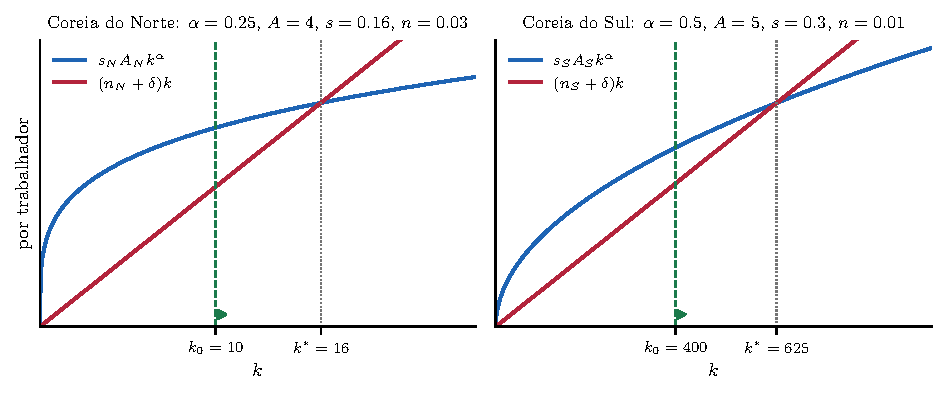
\includegraphics[width=\textwidth]{fig/fig_l2q1_solow.pdf}
\end{center}

%---------------------------------------------------------------- (c)
\subsection*{(c) Unificação com a tecnologia do Sul}

\passo{Passo 1 --- A economia unificada.} Somam-se os estoques; a tecnologia é a do Sul:
$$K_U = 8000 + 100 = 8100, \qquad L_U = 20 + 10 = 30,
\qquad k_U = \frac{8100}{30} = \resp{270}$$
$$y_U = A_S\, k_U^{\alpha_S} = 5\sqrt{270} = \resp{82{,}1584},
\qquad Y_U = 82{,}1584 \times 30 = \resp{2464{,}75}$$
\emph{Verificação por outro caminho:} $Y_U = A_S K_U^{0{,}5} L_U^{0{,}5}
= 5\sqrt{8100}\sqrt{30} = 5 \times 90 \times 5{,}4772 = 2464{,}75$. \checkmark

\passo{Passo 2 --- A mudança no PIB per capita de cada país.}

\begin{center}
\small
\begin{tabular}{lccc}
\toprule
 & $y$ antes & $y$ depois & variação \\
\midrule
Coreia do \textbf{Norte} & $7{,}1131$ & $82{,}1584$
  & \resp{$+1055{,}0\%$} \; ($\times 11{,}55$) \\
Coreia do \textbf{Sul}   & $100{,}00$ & $82{,}1584$
  & \resp{$-17{,}84\%$} \; ($\times 0{,}8216$) \\
\bottomrule
\end{tabular}
\end{center}

O Norte multiplica seu produto por pessoa por mais de onze; o Sul \textbf{perde} quase um
quinto. Note que a queda do Sul é exatamente
$\left(\frac{270}{400}\right)^{1/2} - 1 = \sqrt{0{,}675}-1 = -17{,}84\%$.

\passo{Passo 3 --- De onde vem o ganho do Norte: dois canais.} Decompõe-se
multiplicativamente, mudando uma coisa de cada vez:
$$\underbrace{7{,}1131}_{4 \cdot 10^{0{,}25}}
\;\xrightarrow[\;\times 1{,}2500\;]{A:\,4\to5}\;
\underbrace{8{,}8914}_{5 \cdot 10^{0{,}25}}
\;\xrightarrow[\;\times 1{,}7783\;]{\alpha:\,0{,}25\to0{,}5}\;
\underbrace{15{,}8114}_{5 \cdot 10^{0{,}5}}
\;\xrightarrow[\;\times 5{,}1962\;]{k:\,10\to270}\;
\underbrace{82{,}1584}_{5 \cdot 270^{0{,}5}}$$
e $1{,}25 \times 1{,}7783 \times 5{,}1962 = 11{,}550$, que é exatamente
$82{,}1584/7{,}1131$. \checkmark

Ou seja: \textbf{o ganho do Norte é sobretudo aprofundamento de capital} (fator $5{,}20$),
não adoção de tecnologia (fator $2{,}22$). E, dentro do canal tecnológico, a maior parte
vem da mudança de $\alpha$, não de $A$.

\begin{tcolorbox}[theorybox, title={Uma ressalva honesta sobre comparar tecnologias com $\alpha$ diferente}]
\small
Como $\alpha_N \ne \alpha_S$, não faz sentido dizer que ``a tecnologia do Sul é melhor''
sem qualificação: a comparação depende de $k$. As duas funções se cruzam onde
$4k^{0{,}25} = 5k^{0{,}5}$, isto é, em $k = (4/5)^4 = 0{,}4096$. Acima disso a do Sul rende
mais --- e os dois países operam em $k \geq 10$, ordens de magnitude acima. Então a
afirmação vale \emph{na região relevante}, e é bom dizer por quê.
\end{tcolorbox}

\passo{Passo 4 --- De onde vem a perda do Sul: diluição de capital, pura.} Para o Sul não
há ganho algum a decompor. A tecnologia é a dele mesmo ($\alpha_S$, $A_S$ --- nada muda) e
$s$ e $\delta$ também. A \emph{única} coisa que mudou é que os $8000$ de capital agora
sustentam $30$ trabalhadores em vez de $20$: $k$ cai de $400$ para $270$. O Sul paga a
conta da unificação em capital.

\passo{Passo 5 --- O produto agregado sobe?} \resp{Sim, e bastante.}
$$Y_{\text{antes}} = 2000 + 71{,}13 = 2071{,}13
\quad\longrightarrow\quad Y_U = 2464{,}75
\qquad \resp{+19{,}0\%}$$

E o ganho agregado também se decompõe em dois canais:
\begin{center}
\small
\begin{tabular}{llr}
\toprule
\textbf{Canal} & \textbf{$Y$} & \textbf{efeito} \\
\midrule
Ponto de partida (cada um com a sua tecnologia)              & $2071{,}13$ & --- \\
1) Norte adota a tecnologia do Sul, ainda com $k_N=10$        & $2158{,}11$ & $+4{,}20\%$ \\
2) capital repartido entre os 30 trabalhadores ($k \to 270$)  & $2464{,}75$ & $+14{,}21\%$ \\
\midrule
\multicolumn{2}{r}{\textbf{total} \; ($1{,}0420 \times 1{,}1421 = 1{,}1901$)}
  & \textbf{$+19{,}0\%$} \\
\bottomrule
\end{tabular}
\end{center}

\passo{Passo 6 --- O canal 2 é a desigualdade de Jensen, literalmente.} Vale a pena ver
isso com precisão, porque é o coração econômico do item. Com \emph{uma} tecnologia comum e
côncava $f$, juntar duas economias entrega $f$ avaliada na média ponderada dos $k$, e a
concavidade garante
$$f\big(\lambda k_N + (1-\lambda)k_S\big) \;\geq\;
\lambda f(k_N) + (1-\lambda) f(k_S),
\qquad \lambda = \frac{L_N}{L_U} = \frac13 .$$
Numericamente, com $f(k) = 5\sqrt{k}$:
$$\underbrace{\tfrac13 (5\sqrt{10}) + \tfrac23 (5\sqrt{400})}_{= \;71{,}937\;\text{(sem juntar o capital)}}
\;<\;
\underbrace{5\sqrt{270}}_{=\;82{,}158\;\text{(juntando)}},
\qquad \frac{82{,}158}{71{,}937} = 1{,}1421$$
--- exatamente o $+14{,}21\%$ do canal 2. \checkmark

O mecanismo é a \textbf{equalização do produto marginal do capital}. Sob a tecnologia do
Sul, $\mathrm{PMgK} = \alpha_S A_S k^{\alpha_S - 1} = 2{,}5/\sqrt{k}$:
$$\mathrm{PMgK}\big|_{k=10} = 0{,}791
\qquad\text{contra}\qquad
\mathrm{PMgK}\big|_{k=400} = 0{,}125 ,$$
uma razão de $6{,}3$ para 1. Mover capital do Sul (onde é abundante e rende pouco) para o
Norte (onde é escasso e rende muito) aumenta o produto total; depois da fusão todos operam
com $\mathrm{PMgK} = 0{,}152$.

\intuicao{A unificação faz duas coisas distintas, e é importante não confundi-las. Primeiro,
transplanta a tecnologia melhor para o Norte --- efeito pequeno aqui ($+4{,}2\%$ do
agregado). Segundo, e maior, permite que o capital seja usado onde seu retorno é alto. O
agregado sobe $19\%$, mas a distribuição é brutalmente assimétrica: o Norte multiplica seu
produto por pessoa por $11{,}6$, e o Sul perde $17{,}8\%$. \textbf{Unificação eleva o bolo e
não é Pareto-superior} --- só se torna aceitável para o Sul com transferências, que é
precisamente o que aconteceu na reunificação alemã, onde o Ocidente transferiu somas
enormes para o Oriente durante décadas.}

\refbib{Kurlat (2020), §4.1 ``Ingredients of the Model'' (p.\ 53) e §4.2 ``Mechanics''
(pp.\ 57--60) para a mecânica e a estática comparativa; §4.4 ``Markets'' (p.\ 63) para o
$\mathrm{PMgK}$ como preço de aluguel do capital. Para a velocidade de convergência
formalizada, Romer (2012, 4\textordfeminine{} ed.), cap.\ 1, §1.5.}

%---------------------------------------------------------------- (d)
\subsection*{(d) \textit{Bônus} --- o estado estacionário da Coreia unificada}

\passo{Passo 1 --- Os parâmetros da economia unificada.} Poupança e tecnologia são as do
Sul; a demografia é a média ponderada \emph{pelo trabalho}:
$$s_U = s_S = 0{,}30, \qquad \alpha_U = 0{,}5, \qquad A_U = 5,$$
$$n_U = \frac{L_N n_N + L_S n_S}{L_N + L_S}
= \frac{10(0{,}03) + 20(0{,}01)}{30} = \frac{0{,}5}{30} = \frac{1}{60}
\approx \resp{1{,}667\%}$$

\passo{Passo 2 --- O estado estacionário.} Com $n_U + \delta = \frac{1}{60} + \frac{3}{60}
= \frac{4}{60} = \frac{1}{15}$:
$$\frac{s_U A_U}{n_U+\delta} = \frac{1{,}5}{1/15} = 22{,}5
\quad\Longrightarrow\quad
k\ststst_U = 22{,}5^2 = \resp{506{,}25},
\qquad y\ststst_U = 5\sqrt{506{,}25} = 5(22{,}5) = \resp{112{,}5}$$

\passo{Passo 3 --- Ainda abaixo do estado estacionário?} \resp{Sim, e por muito.}
$$k_U = 270 \quad\text{contra}\quad k\ststst_U = 506{,}25
\qquad \Longrightarrow \qquad \frac{k_U}{k\ststst_U} = 53{,}3\%$$
Em termos de produto, $y_U = 82{,}16$ contra $y\ststst_U = 112{,}5$, ou $73{,}0\%$. A Coreia
unificada acorda no dia seguinte à fusão com pouco mais da metade do capital por
trabalhador que terá no longo prazo, e portanto cresce por várias décadas ainda.

\passo{Passo 4 --- $y\ststst_U$ contra $y\stst_S$: a comparação que a questão quer.}
$$y\ststst_U = 112{,}5 \qquad\text{contra}\qquad y\stst_S = 125
\qquad\Longrightarrow\qquad \frac{y\ststst_U}{y\stst_S} = 0{,}90
\quad \resp{-10\%}$$

\textbf{A explicação é limpa porque só um parâmetro mudou.} A economia unificada herdou
$s$, $A$ e $\alpha$ do Sul --- idênticos. A \emph{única} diferença em relação ao Sul
isolado é $n$: subiu de $1\%$ para $1{,}667\%$, porque o Norte trouxe sua demografia mais
acelerada para a média. E $n$ mais alto significa mais \textbf{diluição de capital}: mais
trabalhadores novos para equipar a cada ano, logo uma reta de reposição $(n+\delta)k$ mais
íngreme, logo $k\stst$ e $y\stst$ menores. Formalmente,
$$\frac{y\ststst_U}{y\stst_S}
= \left(\frac{n_S+\delta}{n_U+\delta}\right)^{\frac{\alpha}{1-\alpha}}
= \left(\frac{0{,}06}{1/15}\right)^{1} = 0{,}90 ,$$
onde o expoente vale exatamente $1$ porque $\alpha = 0{,}5$. \checkmark

\begin{center}
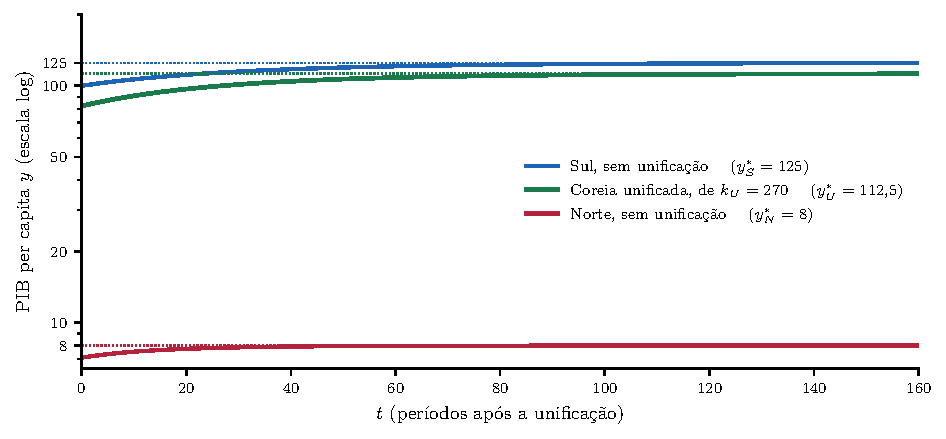
\includegraphics[width=\textwidth]{fig/fig_l2q1_trajetorias.pdf}
\end{center}

\passo{Passo 5 --- Juntando tudo: quem ganha e quem perde, no curto e no longo prazo.}

\begin{center}
\small
\begin{tabular}{lcccc}
\toprule
 & \multicolumn{2}{c}{\textbf{no impacto}} & \multicolumn{2}{c}{\textbf{no longo prazo}} \\
\cmidrule(lr){2-3}\cmidrule(lr){4-5}
 & sem unificar & unificado & sem unificar & unificado \\
\midrule
Norte & $7{,}11$  & $82{,}16$ \; ($\times11{,}55$)
      & $8$       & $112{,}5$ \; ($\times14{,}06$) \\
Sul   & $100{,}0$ & $82{,}16$ \; ($-17{,}8\%$)
      & $125$     & $112{,}5$ \; ($-10{,}0\%$) \\
\midrule
média ponderada & $71{,}0$ & $82{,}16$ \; ($+15{,}7\%$)
                & $86{,}0$ & $112{,}5$ \; ($+30{,}8\%$) \\
\bottomrule
\end{tabular}
\end{center}

O sul-coreano perde \emph{duas vezes}: imediatamente e para sempre. O norte-coreano ganha
uma ordem de magnitude nas duas margens. Na média ponderada, a unificação eleva o $y\stst$
coreano de $86$ para $112{,}5$ ($+30{,}8\%$) --- o ganho de eficiência é real, mas quem o
recebe não é quem o paga. E o crescimento agregado de longo prazo passa a ser
$g_Y = n_U = 1{,}667\%$, entre o $1\%$ do Sul e o $3\%$ do Norte.

\begin{tcolorbox}[rubricbox]
\small
\textbf{(a)} 0,6 --- os quatro números ($k_0$ e $y_0$ dos dois países); derivar
$y = Ak^{\alpha}$ conta.
\textbf{(b)} 1,2 --- derivação de $k\stst$ com os passos algébricos (0,5); os quatro valores
(0,3); resposta sobre crescimento, incluindo \emph{explicitamente} que não há convergência
entre os países (0,4).
\textbf{(c)} 1,4 --- $k_U$ e $y_U$ (0,4); variação para cada país, com os dois sinais
corretos (0,4); origem do ganho/perda em cada caso (0,3); agregado sobe, com a conta (0,3).
\textbf{(d)} 0,8 --- $n_U$ ponderado \emph{pelo trabalho} (0,2); $k\ststst_U$ e
$y\ststst_U$ (0,3); ainda abaixo do estado estacionário (0,1); $y\ststst_U < y\stst_S$
atribuído a $n$ (0,2).

\smallskip
\textbf{Tetos por erro conceitual} (prevalecem sobre penalidades leves, não se somam):
\begin{itemize}[topsep=2pt]
\item Concluir em (b) que o Norte converge para o nível do Sul por ser mais pobre:
      máx.\ 0,5 no item. Os estados estacionários são \emph{diferentes}.
\item Dizer em (b) que há crescimento de $y$ no longo prazo (não há progresso tecnológico):
      máx.\ 0,6 no item.
\item Em (c), calcular $y_U$ como média de $y_N$ e $y_S$ em vez de reavaliar
      $A_S k_U^{\alpha_S}$: 0 no item --- é ignorar a concavidade, que é o ponto todo.
\item Em (c), afirmar que o Sul também ganha: máx.\ 0,6 no item.
\item Em (d), usar média simples de $n_N$ e $n_S$ ($2\%$) em vez da ponderada pelo trabalho
      ($1{,}667\%$): $-0{,}3$.
\item Em (d), atribuir $y\ststst_U < y\stst_S$ a diferença de tecnologia ou de poupança:
      máx.\ 0,4 no item --- só $n$ mudou.
\item Escrever a reta de reposição como $\delta k$, esquecendo $n$: máx.\ 1,5 na questão.
\end{itemize}
\textbf{Penalidade leve:} erro aritmético com método correto, $-0{,}2$.

\smallskip
\textbf{Risco residual:} os números foram construídos para sair exatos
($16$, $625$, $506{,}25$, $8$, $125$, $112{,}5$). Se o seu $k\stst$ saiu quebrado, o erro
mais provável é ter usado $\left(\frac{s}{n+\delta}\right)^{1/(1-\alpha)}$
\textbf{esquecendo o $A$} dentro do numerador.
\end{tcolorbox}

%======================================================================
\section[Questão 2 --- Gotham: capital de segurança e PTF medida]{Questão 2 \quad Gotham: capital de segurança e PTF medida \hfill \normalsize (6 pontos)}
%======================================================================

\begin{tcolorbox}[questionbox]
\small
In the city of Gotham the production function is $Y = A K_P^{\alpha} L^{1-\alpha}$
\hfill (1)\\
where $K_P$ is capital used in production. Factor markets are perfectly competitive and the
price of output is normalized to 1. Unfortunately, crime is a significant problem in Gotham,
so for each unit of productive capital, firms need to invest $\theta$ units of capital in
security (i.e., cameras, armored cars, and masked vigilantes). This ratio is fixed, and
security capital is recorded in the national accounts as capital, alongside productive
capital. Use $K$ to denote the \textit{total} capital stock, as opposed to $K_P$. Where a
numerical answer is requested, use $\alpha = 1/3$ and $\theta = 0.5$.

\smallskip
\textbf{(a)} Find an expression for total output as a function of $A, K, L, \theta$ and
$\alpha$. What fraction of the measured capital stock is devoted to security? How much
output is lost due to the need for security?
\textbf{(b)} Write down and solve the problem of a firm that chooses $K_P$ and $L$ to
maximize profits, taking $w$ and $r$ as given. Notice that the firm has to pay the same
rental rate on security capital as on productive capital and compute the factor shares that
a statistical agency would measure. Are they distorted by the presence of crime?
\textbf{(c)} Suppose a "riddler" applies the development accounting exercise of
\textbf{Kurlat Section 5.3}. They observe $Y$, $K$ and $L$ accurately, but cannot separate
productive from security capital pool them together. What estimate of productivity
$\hat{A}$ do they obtain, and how does it compare to the true value of $A$? In light of item
(b), is the riddler's value of $\alpha$ also wrong?
\textbf{(d)} WayneTech invents a new security technology which reduces the security capital
requirement from $\theta$ to $\theta' = \frac{1}{4}\theta$. Suppose the transition takes
place over a decade, during which the total capital stock grows at $g_K$ and the labor force
at $g_L$. Using equation (5.4.2), write out the growth accounting decomposition of $g_Y$ and
solve for the Solow residual. True technology $A$ has not changed at all: show that the
entire effect of the new technology is reported as TFP growth, and compute the implied
annual rate numerically. Explain why this is consistent with Kurlat's statement that the
residual captures ``changes in policies that lead to better (or worse) allocation of
resources'', and state what the accounting exercise would report if instead crime had
worsened.
\end{tcolorbox}

\begin{tcolorbox}[theorybox, title={O arco da questão --- vale ler antes de começar}]
\small
Os quatro itens montam um argumento único, e cada um depende do anterior:
(a) o crime é algebricamente idêntico a um \textbf{redutor de PTF};
(b) apesar disso, ele \textbf{não distorce as participações dos fatores};
(c) logo o econometrista acerta $\alpha$ e erra $A$ --- toda a cunha aparece como
``atraso tecnológico'';
(d) e como as participações estão certas, a contabilidade do crescimento joga
\emph{todo} o efeito de uma reforma de segurança no resíduo de Solow.
O item (b) é o que faz (c) e (d) funcionarem; não o trate como um cálculo mecânico.
\end{tcolorbox}

%---------------------------------------------------------------- (a)
\subsection*{(a) Produto total, composição do capital e perda de produto}

\passo{Passo 1 --- Separar capital total de capital produtivo.} Por cada unidade de capital
produtivo é preciso $\theta$ unidades de segurança, então
$$K = \underbrace{K_P}_{\text{produtivo}} + \underbrace{\theta K_P}_{\text{segurança}}
= (1+\theta)K_P
\qquad\Longrightarrow\qquad K_P = \frac{K}{1+\theta}$$

\passo{Passo 2 --- Substituir em (1).}
$$Y = A K_P^{\alpha}L^{1-\alpha}
= A\left(\frac{K}{1+\theta}\right)^{\alpha} L^{1-\alpha}
\qquad\Longrightarrow\qquad
\boxed{\;Y = \underbrace{A\,(1+\theta)^{-\alpha}}_{\text{PTF \emph{efetiva}}}
K^{\alpha}L^{1-\alpha}\;}$$

Guarde este resultado: escrita em termos do capital \textbf{medido} $K$, a economia de
Gotham é uma Cobb-Douglas normal com o \emph{mesmo} $\alpha$ e uma produtividade
multiplicada por $(1+\theta)^{-\alpha} < 1$. \textbf{O crime entra exatamente como um
imposto sobre a PTF} --- e é disso que vivem os itens (c) e (d).

\passo{Passo 3 --- Fração do capital medido em segurança.}
$$\frac{K_{\text{seg}}}{K} = \frac{\theta K_P}{(1+\theta)K_P}
= \frac{\theta}{1+\theta} = \frac{0{,}5}{1{,}5} = \resp{\frac13 \approx 33{,}3\%}$$
e portanto $1/(1+\theta) = 2/3$ do estoque medido é produtivo.

\passo{Passo 4 --- Quanto de produto se perde.} A comparação natural é contra uma Gotham
sem crime que dispusesse do \emph{mesmo} estoque total $K$, todo ele produtivo:
$$\frac{Y(\theta)}{Y(\theta=0)} = (1+\theta)^{-\alpha} = 1{,}5^{-1/3}
= \resp{0{,}8736}
\qquad\Longrightarrow\qquad \text{perdem-se } \resp{12{,}64\%} \text{ do produto.}$$

\textbf{Note a assimetria, que é o ponto quantitativo do item:} um terço do capital está
improdutivo, mas o produto cai apenas $12{,}6\%$ --- não $33\%$. A razão é que a
elasticidade do produto ao capital é só $\alpha = 1/3$:
$$\ln\frac{Y(\theta)}{Y(0)} = \alpha \ln\frac{K_P}{K}
= \tfrac13 \ln \tfrac23 = \tfrac13(-0{,}4055) = -0{,}1352,
\qquad e^{-0{,}1352} = 0{,}8736 . \; \checkmark$$
Perder um terço do capital custa um terço \emph{de um terço} em logs.

\emph{Leitura alternativa, que vale mencionar:} se em vez disso comparássemos com uma
Gotham que mantivesse o mesmo $K_P$, o produto seria idêntico e a economia estaria em
recursos --- pouparia $\theta K_P = K/3$ de capital. As duas leituras são coerentes; a
primeira responde ``quanto produto se perde'', que é o que foi perguntado.

\begin{center}
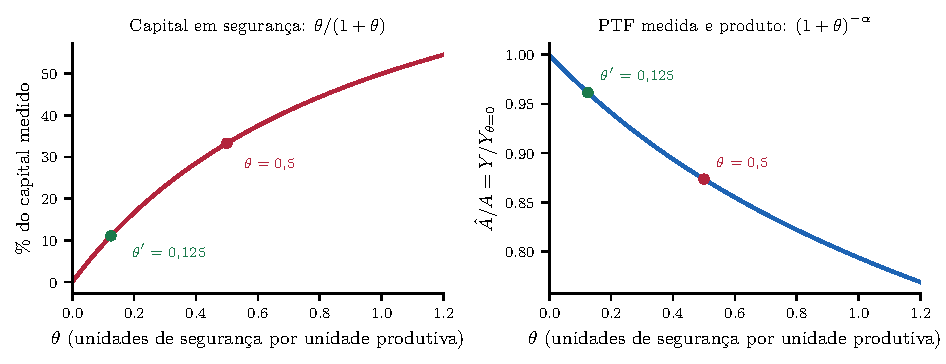
\includegraphics[width=\textwidth]{fig/fig_l2q2_crime.pdf}
\end{center}

%---------------------------------------------------------------- (b)
\subsection*{(b) O problema da firma e as participações medidas}

\passo{Passo 1 --- Montar o problema com o custo \emph{correto} do capital.} A firma que
quer $K_P$ unidades produtivas é obrigada a comprar $(1+\theta)K_P$ unidades de capital, e
paga $r$ sobre \emph{todas} --- o enunciado é explícito nisso. Com o preço do produto
normalizado em 1:
$$\max_{K_P,\,L} \;\; \pi = A K_P^{\alpha}L^{1-\alpha}
\;-\; r\,(1+\theta)K_P \;-\; wL$$

\passo{Passo 2 --- Condições de primeira ordem.}
$$\frac{\partial \pi}{\partial K_P} = 0:
\qquad \alpha A K_P^{\alpha-1}L^{1-\alpha} = r(1+\theta)
\qquad\Longleftrightarrow\qquad \alpha\,\frac{Y}{K_P} = r(1+\theta)$$
$$\frac{\partial \pi}{\partial L} = 0:
\qquad (1-\alpha)A K_P^{\alpha}L^{-\alpha} = w
\qquad\Longleftrightarrow\qquad w = (1-\alpha)\frac{Y}{L}$$

Agora o passo que faz a mágica. Da primeira CPO, isole $r$ e use $(1+\theta)K_P = K$:
$$r = \frac{\alpha Y}{(1+\theta)K_P} = \boxed{\;\alpha\,\frac{Y}{K}\;}$$
O produto marginal do capital \emph{produtivo} é $\alpha Y/K_P$, maior que $\alpha Y/K$;
mas o retorno que a firma consegue pagar por unidade de capital \emph{medido} é $\alpha Y/K$,
porque cada unidade produtiva arrasta $\theta$ unidades de vigilância junto.

\passo{Passo 3 --- As participações que uma agência estatística mediria.}
\begin{align*}
\text{participação do capital} &= \frac{rK}{Y}
  = \frac{\left(\alpha Y/K\right)K}{Y} = \resp{\alpha = \tfrac13},\\[2pt]
\text{participação do trabalho} &= \frac{wL}{Y}
  = \frac{\left((1-\alpha)Y/L\right)L}{Y} = \resp{1-\alpha = \tfrac23}.
\end{align*}

\resp{As participações NÃO são distorcidas pelo crime.} E, coerentemente,
$\pi = Y - rK - wL = Y - \alpha Y - (1-\alpha)Y = 0$: lucro zero, como tem de ser sob
retornos constantes de escala e concorrência perfeita.

\passo{Passo 4 --- Por que isso tinha de acontecer.} Não é coincidência algébrica. Pelo
item (a), em termos dos fatores \emph{medidos} $(K,L)$ a tecnologia de Gotham é
$$Y = \big[A(1+\theta)^{-\alpha}\big] K^{\alpha}L^{1-\alpha},$$
uma Cobb-Douglas com expoente $\alpha$ em $K$ e uma constante multiplicativa. Sob
Cobb-Douglas as participações dos fatores igualam os \textbf{expoentes}, e não dependem do
nível da PTF. O crime desloca a constante e deixa os expoentes intactos --- logo é
\textbf{invisível} nas participações. É uma função homogênea de grau 1 em $(K,L)$, e o
teorema de Euler faz o resto.

\intuicao{Esta é a observação mais importante da questão. Existe uma ineficiência enorme na
economia --- um terço do capital produzindo nada --- e ela \emph{não deixa impressão
digital} nos dados de distribuição de renda. Quem só olha participações de fatores conclui
que Gotham é uma economia competitiva normal com $\alpha = 1/3$, e está certo nisso. A
distorção está toda em outro lugar, e os itens (c) e (d) mostram onde.}

%---------------------------------------------------------------- (c)
\subsection*{(c) O \emph{riddler} e a produtividade medida}

\passo{Passo 1 --- O que o riddler faz.} Ele observa $Y$, $K$ e $L$ corretamente, mas não
consegue separar $K_P$ de $K_{\text{seg}}$ --- e, como o enunciado avisa, as contas
nacionais registram os dois juntos como capital. Então ele supõe a especificação padrão do
Kurlat §5.3 e inverte para a produtividade:
$$Y = \hat{A}\, K^{\alpha}L^{1-\alpha}
\qquad\Longrightarrow\qquad
\hat{A} = \frac{Y}{K^{\alpha}L^{1-\alpha}}$$

\passo{Passo 2 --- Comparar com a verdade.} Substituindo o $Y$ verdadeiro do item (a):
$$\hat{A} = \frac{A(1+\theta)^{-\alpha}K^{\alpha}L^{1-\alpha}}{K^{\alpha}L^{1-\alpha}}
\qquad\Longrightarrow\qquad
\boxed{\;\hat{A} = A\,(1+\theta)^{-\alpha}\;}$$
$$\frac{\hat A}{A} = 1{,}5^{-1/3} = \resp{0{,}8736}
\qquad\Longrightarrow\qquad
\text{o riddler \textbf{subestima} } A \text{ em } \resp{12{,}64\%}.$$

\passo{Passo 3 --- E o $\alpha$ dele, está errado?} \resp{Não --- o $\alpha$ está correto.}
E é o item (b) que garante isso. Em development accounting, $\alpha$ não é estimado por
regressão: é \textbf{calibrado pela participação do capital na renda} observada. O item (b)
mostrou que essa participação é exatamente $\alpha$. Logo o riddler lê $1/3$ nas contas
nacionais, usa $1/3$, e acerta.

\resp{Consequência: todo o erro se concentra na PTF.} Não há nenhuma combinação de dados
de produto, capital, trabalho e participações que revele a existência do crime. Só
observando a \emph{composição} do estoque de capital --- quanto é câmera e quanto é
máquina --- se descobriria o problema.

\intuicao{É exatamente a moral do §5.3 do Kurlat, e o motivo de a Conjectura 5.1 ser
rejeitada. O riddler conclui que Gotham é ``tecnologicamente atrasada''. Mas não há nada de
errado com a função de produção de Gotham: o que há é um terço do estoque de capital
vigiando os outros dois terços. Chamar isso de baixa PTF é contabilmente correto e
economicamente enganoso --- e é a razão pela qual a literatura moderna lê boa parte dos
hiatos de PTF entre países como \textbf{má alocação de recursos e instituições}, não como
ignorância técnica. Gotham não precisa de um inventor; precisa de polícia.}

\refbib{Kurlat (2020), §5.3 ``The Capital Accumulation Hypothesis'' (pp.\ 80--85) --- a
Conjectura 5.1 e a Fig.\ 5.3.3, que compara o PIB per capita previsto pelo capital com o
observado; §5.5 ``Where do TFP differences come from?'' (pp.\ 89--92) para a leitura da PTF
como instituições e alocação.}

%---------------------------------------------------------------- (d)
\subsection*{(d) WayneTech: a reforma que aparece como progresso técnico}

\passo{Passo 1 --- A equação (5.4.2) do Kurlat.} Partindo de $Y_t = F(K_t,L_t,A_t)$ e
tomando uma aproximação de primeira ordem, Kurlat obtém
\begin{equation*}
g_Y \;=\;
\underbrace{\frac{F_K K_t}{F}}_{\text{part.\ do capital}}
\underbrace{\frac{K_{t+1}-K_t}{K_t}}_{g_K}
\;+\;
\underbrace{\frac{F_L L_t}{F}}_{\text{part.\ do trabalho}}
\underbrace{\frac{L_{t+1}-L_t}{L_t}}_{g_L}
\;+\;
\underbrace{\frac{F_A A_t}{F}\frac{A_{t+1}-A_t}{A_t}}_{\text{resíduo de Solow}}
\tag{5.4.2}
\end{equation*}
de onde, resolvendo para o termo não observável,
$$\text{Resíduo de Solow} = g_Y
- (\text{part.\ do capital})\, g_K - (\text{part.\ do trabalho})\, g_L .$$

\textbf{É aqui que o item (b) entra.} A agência usa as participações \emph{medidas} como
pesos --- e o item (b) provou que elas valem exatamente $\alpha$ e $1-\alpha$. Portanto os
pesos estão \emph{certos}, e nenhuma parte do efeito do crime é indevidamente atribuída à
acumulação de fatores.

\passo{Passo 2 --- Escrever a decomposição para Gotham.} Do item (a),
$Y_t = A(1+\theta_t)^{-\alpha}K_t^{\alpha}L_t^{1-\alpha}$. Tomando logaritmos e diferenças
ao longo da década (o que é a versão exata da aproximação de (5.4.2)):
$$\Delta \ln Y = \underbrace{\Delta \ln A}_{=\;0}
\;-\; \alpha\,\Delta\ln(1+\theta)
\;+\; \alpha\,\Delta \ln K
\;+\; (1-\alpha)\Delta \ln L$$

\passo{Passo 3 --- Resolver para o resíduo.} Por definição, o resíduo é o que sobra depois
de descontar a acumulação de fatores com os pesos $\alpha$ e $1-\alpha$:
$$\Delta\ln\hat A \;=\; \Delta \ln Y - \alpha\,\Delta\ln K - (1-\alpha)\Delta \ln L
\;=\; -\alpha\,\Delta \ln(1+\theta)$$
$$\boxed{\;\Delta \ln \hat A
= \alpha \ln\!\left(\frac{1+\theta}{1+\theta'}\right)\;}$$

\resp{Este é o resultado que o item pede.} Duas leituras imediatas:

\begin{itemize}
\item \textbf{$A$ não mudou e o resíduo é positivo.} Por hipótese $\Delta \ln A = 0$: a
tecnologia de produção é a mesma. Ainda assim o resíduo é estritamente positivo, e
\emph{todo} o efeito da inovação da WayneTech é reportado como crescimento da PTF.
\item \textbf{O resíduo não depende de $g_K$ nem de $g_L$.} Os termos de acumulação foram
subtraídos exatamente com os pesos corretos, então o efeito de $\theta$ é ortogonal a eles.
Não importa se o capital cresceu $0\%$ ou $10\%$ ao ano --- o resíduo é o mesmo.
(Verificado numericamente para quatro pares $(g_K,g_L)$ distintos. \checkmark)
\end{itemize}

\passo{Passo 4 --- A conta numérica.} Com $\theta = 0{,}5$ e
$\theta' = \tfrac14\theta = 0{,}125$:
$$\frac{1+\theta}{1+\theta'} = \frac{1{,}5}{1{,}125} = \frac43$$
$$\Delta\ln\hat A = \tfrac13 \ln\tfrac43 = \tfrac13(0{,}28768) = 0{,}09589
\qquad\Longrightarrow\qquad
\frac{\hat A'}{\hat A} = \left(\tfrac43\right)^{1/3} = 1{,}1006$$

Ou seja, a PTF medida sobe \resp{$+10{,}06\%$ ao longo da década}. Anualizando:
$$\text{taxa composta} = \left(\tfrac43\right)^{1/30} - 1 = \resp{0{,}964\%\text{ ao ano}}
\qquad\big(\text{em log: } 0{,}09589/10 = 0{,}959\%\text{ ao ano}\big)$$

Para dar contexto: quase um ponto percentual anual de ``progresso tecnológico'' durante dez
anos, sem que uma única função de produção tenha mudado. Enquanto isso, a composição do
capital medido se desloca de $33{,}3\%$ para $\theta'/(1+\theta') = 11{,}1\%$ em segurança
--- e de $66{,}7\%$ para $88{,}9\%$ em uso produtivo.

\passo{Passo 5 --- Por que isso é coerente com a frase do Kurlat.} O resíduo de Solow é
\emph{definido} como tudo aquilo no crescimento do produto que não é explicado pelos
fatores \textbf{medidos}. A reforma da WayneTech não criou capital nem trabalho: ela
\textbf{realocou} o estoque existente, de vigiar para produzir. Como $K$ e $L$ medidos não
se movem por causa disso, o ganho não tem para onde ir a não ser o resíduo.

Então a frase de Kurlat --- que o resíduo captura ``changes in policies that lead to better
(or worse) allocation of resources'' --- não é uma ressalva de rodapé: é uma descrição
literal do que aconteceu aqui. E vale insistir num ponto que é fácil errar: esse
crescimento de PTF é \textbf{genuíno e relevante para o bem-estar}. Gotham realmente produz
$10\%$ mais com os mesmos insumos medidos. O que ele \emph{não} é é invenção. ``PTF'' é o
nome de uma medida residual, não de uma tecnologia.

\passo{Passo 6 --- E se o crime tivesse \emph{piorado}?} O sinal simplesmente se inverte, e
essa simetria é o teste final da lógica. Suponha $\theta$ subindo de $0{,}5$ para
$\theta'' = 4\theta = 2$ na mesma década:
$$\frac{1+\theta}{1+\theta''} = \frac{1{,}5}{3} = \frac12,
\qquad
\Delta\ln\hat A = \tfrac13\ln\tfrac12 = -0{,}2310$$
$$\Longrightarrow\quad \hat A \text{ cai } \resp{20{,}63\%} \text{ na década},
\text{ ou } \resp{-2{,}28\%\text{ ao ano}}$$

\resp{O exercício reportaria regresso tecnológico} --- PTF negativa, uma economia
``desaprendendo'' a produzir --- quando na verdade $A$ nunca se moveu e o que houve foi
deterioração institucional. É precisamente assim que se leem os colapsos medidos de PTF em
episódios de conflito, insegurança ou ruptura institucional: não como esquecimento
tecnológico, mas como recursos desviados para atividades defensivas.

\refbib{Kurlat (2020), §5.4 ``Growth Accounting'' (pp.\ 86--88) --- a equação (5.4.2), a
definição do resíduo e a frase citada, todas na p.\ 87; §5.3 (pp.\ 80--85) para o exercício
de níveis do item (c). Complementar: Jones (2020, 5\textordfeminine{} ed.), cap.\ 6, para a
mesma contabilidade com dados.}

\begin{tcolorbox}[rubricbox]
\small
\textbf{(a)} 1,5 --- $K_P = K/(1+\theta)$ e a expressão
$Y = A(1+\theta)^{-\alpha}K^{\alpha}L^{1-\alpha}$ (0,7); fração $\theta/(1+\theta) = 1/3$
(0,4); perda $1-(1+\theta)^{-\alpha} = 12{,}64\%$ (0,4).
\textbf{(b)} 1,5 --- problema com o custo $r(1+\theta)K_P$ (0,4); as duas CPO (0,4);
$r = \alpha Y/K$ (0,3); participações $=(\alpha,1-\alpha)$ e resposta explícita ``não são
distorcidas'' (0,4).
\textbf{(c)} 1,5 --- $\hat A = A(1+\theta)^{-\alpha}$ (0,6); comparação numérica com $A$
(0,3); $\alpha$ correto \emph{porque} vem da participação medida em (b) (0,6).
\textbf{(d)} 1,5 --- escrever (5.4.2) com as participações medidas (0,3); resíduo
$= \alpha\ln\frac{1+\theta}{1+\theta'}$ (0,4); taxa anual $\approx 0{,}96\%$ (0,3);
conexão com a frase sobre alocação de recursos (0,3); sinal invertido se o crime piorasse
(0,2).

\smallskip
\textbf{Tetos por erro conceitual:}
\begin{itemize}[topsep=2pt]
\item Em (a), responder que a perda de produto é $33\%$ (confundir fração do capital com
      fração do produto): máx.\ 0,8 no item.
\item Em (b), fazer a firma pagar $r$ só sobre $K_P$: derruba (b) para máx.\ 0,5
      \emph{e} contamina (c) e (d) --- é a hipótese central do enunciado.
\item Em (b), concluir que as participações \emph{são} distorcidas: máx.\ 0,7 no item.
\item Em (c), afirmar que o $\alpha$ do riddler também está errado sem notar que ele é
      calibrado pela participação: máx.\ 0,9 no item.
\item Em (d), atribuir o resíduo a progresso técnico verdadeiro: máx.\ 0,8 no item.
\item Em (d), fazer o resíduo depender de $g_K$ e $g_L$: $-0{,}4$.
\end{itemize}
\textbf{Bônus de completude:} notar que o resíduo é \emph{independente} de $g_K$ e $g_L$, e
que a PTF medida em (c) é numericamente a mesma coisa que a perda de produto em (a) --- não
é coincidência, é a mesma expressão $(1+\theta)^{-\alpha}$ vista de dois ângulos.
\end{tcolorbox}

%======================================================================
\section*{Síntese --- o fio que liga as duas questões}
\addcontentsline{toc}{section}{Síntese}
%======================================================================

\begin{tcolorbox}[theorybox, title={O que a Lista 2 está realmente testando}]
\small
As duas questões atacam, de lados opostos, a mesma pergunta: \emph{por que alguns lugares
produzem mais que outros?}

\begin{itemize}
\item \textbf{Questão 1 --- a resposta ``capital''.} Dois países com os mesmos ingredientes
qualitativos e parâmetros diferentes convergem para estados estacionários diferentes: o
hiato de $15{,}6$ vezes entre as Coreias é \textbf{permanente}, não transitório. E quando
se permite ao capital cruzar a fronteira (a unificação), o ganho agregado de $19\%$ vem em
boa parte de \textbf{realocar} capital para onde o $\mathrm{PMgK}$ é alto --- pura
concavidade, pura desigualdade de Jensen.
\item \textbf{Questão 2 --- a resposta ``PTF''.} Uma economia pode ter a tecnologia certa,
o $\alpha$ certo e mercados competitivos, e ainda assim medir $12{,}6\%$ menos
produtividade, só porque um terço do seu capital está imobilizado em atividade defensiva. A
cunha é invisível nas participações dos fatores e visível apenas no resíduo.
\end{itemize}

Juntas, elas entregam a mensagem do cap.\ 5: \textbf{a PTF medida não é ``tecnologia'' ---
é o nome do que sobrou}, e boa parte do que sobra é alocação de recursos. A Questão 1
mostra má alocação \emph{entre} países (capital preso no Sul); a Questão 2, má alocação
\emph{dentro} de um país (capital preso em vigilância). O mecanismo é o mesmo nas duas.

\smallskip
\textbf{As três armadilhas mais caras da lista:} (i) concluir na Q1(b) que o Norte converge
para o Sul; (ii) responder na Q1(c) que a unificação é boa para os dois países; (iii) dizer
na Q2(b) que o crime distorce as participações dos fatores --- erro que, além do próprio
item, inviabiliza (c) e (d). Somadas, valem cerca de 3 pontos.
\end{tcolorbox}

%======================================================================
\section*{Apêndice \quad Código}
\addcontentsline{toc}{section}{Apêndice --- Código}
%======================================================================

Os scripts estão em \texttt{Resolucao/lista2\_codigo/} e rodam com \texttt{numpy} e
\texttt{matplotlib} (sem dados externos --- a Lista 2 é toda analítica).

\begin{center}
\small
\begin{tabular}{llp{7.2cm}}
\toprule
\textbf{Arquivo} & \textbf{Questão} & \textbf{O que faz} \\
\midrule
\texttt{l2q1\_coreia.py}  & 1 & Todos os números da Q1. Usa \texttt{Fraction} para
  $k_0$, $k_U$ e $n_U$ (exatos), confirma cada $k\stst$ como ponto fixo da lei de
  movimento, e verifica as duas decomposições do item (c) contra o cálculo direto. \\
\texttt{l2q2\_gotham.py}  & 2 & Todos os números da Q2. Confere as CPO da firma, mostra
  participações $=(\alpha,1-\alpha)$ com lucro zero, e verifica que o resíduo de Solow é
  invariante a $(g_K,g_L)$ para quatro pares distintos. \\
\texttt{l2\_figuras.py}   & 1, 2 & Gera as três figuras. \\
\texttt{estilo\_mpl.py}   & --- & Backend \texttt{pgf} (texto das figuras em fontes
  Type 1) e largura casada com a do texto, para inclusão em escala 1:1. \\
\bottomrule
\end{tabular}
\end{center}

\passo{Reprodução.}

\begin{tcolorbox}[colback=gray!7, colframe=gray!50, arc=2pt, boxrule=0.4pt]
\footnotesize
\begin{verbatim}
python l2q1_coreia.py    # itens (a)-(d) da Questao 1, com verificacoes
python l2q2_gotham.py    # itens (a)-(d) da Questao 2, com verificacoes
python l2_figuras.py     # fig_l2q1_solow, fig_l2q1_trajetorias, fig_l2q2_crime
\end{verbatim}
\end{tcolorbox}

\end{document}
